\chapter{State of the Art}
\section{Introduction}

In order to quantify internet censorship conducted across the globe it is important to understand the different methods used by censors to achieve their aims. Censors engage in a range of steps at various layers of the OSI model in order to either stop the publication of information or make it more difficult for the user to attain. Ultimately, a censors choice of how they detect and interrupt the flow of undesirable information is based on a number of factors such as cost, scalability, and whether the censor wishes to be transparent.

Finding comprehensive and credible resources on censorship mechanisms proved challenging due to the depth of the research area. One resource that proved particularly useful in this way were Requests for Comments (RFCs). These documents highlight internet standards placed by the Internet Engineering Task Force and thus provide the accurate technical specifications needed. RFC 9505 proved invaluable in highlighting the majority of censorship methods used today. It was last updated by the Internet Research Task Force in late 2023 and provides the technical basis for this section of the thesis. The document "describes technical mechanisms employed in network censorship that regimes around the world use for blocking or impairing Internet traffic."\cite{rfc9505} In combination with relevant academic papers, other RFCs like 2818 (HTTPS) \cite{rfc2818} and 8446 (TLS 1.3) \cite{rfc8446} were examined.

\subsection{Overt vs. Covert Censorship }
ICLab, a censorship measurement tool very similar to OONI, released a paper in 2020 describing the need for their contribution. In this paper, the author highlights an important distinction between covert and overt censorship: 'In overt censorship, the censor sends the user a 'block page' instead of the material that was censored. In covert censorship, the censor causes a network error that could have occurred for other reasons, and thus avoids informing the user that the material was censored.” \cite{9152784} This is a concerning capability as it alludes to the potential for censorship to go unchecked. 


\section{Censorship Techniques and Mechanisms} 

\subsection{Points of Control}
Key control points are nodes in the Internet’s architecture that connect a large user base to the wider network, making them attractive targets for censorship enforcement. RFC 9505 explains points of control in great detail. It states "internet censorship takes place in all parts of the network topology," however, "There are various logical and physical points of control that censors may use for interception mechanism."\cite{rfc9505}. Below are some notable points of control explained.

Some points of control include ISPs, IXPs, VPNs, national gateways and local networks. These are noteworthy locations where censors likely operate.
Internet Service Providers (ISPs)

Internet Exchange Points (IXPs)

National Gateways

Services

Institutions and Content Sites

Governments and institutions leverage these nodes in the network's topology to restrict user access to undesirable content.  Institutions will typically use a combination of legislative pressure, technological and economic means to snuff out content. ISPs and VPNs face significant and constant pressure from legal arms to expose user data and manipulate the content available to a user. 


In his research paper from 2003, Zittrain gives a solid overview of points of control. He discusses varying reasons to be concerned about points of control and how they are used. One argument he makes is the violation of the end-to-end principle. Simply, this refers to keeping the middle of the network simple and pushing complexity out towards the edge of the network to hosts. 

"The technical aspect of the end-to-end argument suggests a warning against blocking data transmissions at any point [other than endpoints]." \cite{Zittrain_Internet_Points_of_Control}

These locations in the internet infrastructure are invaluable to those wishing to conduct internet censorship. Though security considerations such as HTTPS and TLS can protect users from MITM attacks, points of control are a physical reality to be contended with. At some point, user packets will route through state owned infrastructure and thus could be subject to inspection. In this way, points of control are a key consideration for all internet users. Zittrain concludes his research with a word of warning regarding points of control and their potential for abuse. He highlights the need for "a comprehensive framework where sovereigns’ actions to block material are thoroughly documented and open to challenge." \cite{Zittrain_Internet_Points_of_Control} Unfortunately, we are yet to see this in action since 2003.

\section{Network-Level Filtering }
\subsection{IP and DNS Blocking (GRIFF)}
Communicating on the internet typically looks something like that seen in the figure below. A publisher's website is associated with a domain, e.g www.example.com. A user who wishes to navigate to this site must first send a DNS request to the DNS server to resolve the IP address of the web server. Upon receiving the IP address, the user can then send a HTML get request in order to access the page. How the Domain Name System and Internet Protocol work together to navigate users through a vast infrastructure can thus be simplified into these two transactions. If the censor has access to this DNS server, these flows can be manipulated in a number of ways to disrupt communication.

\begin{figure}
    \centering
    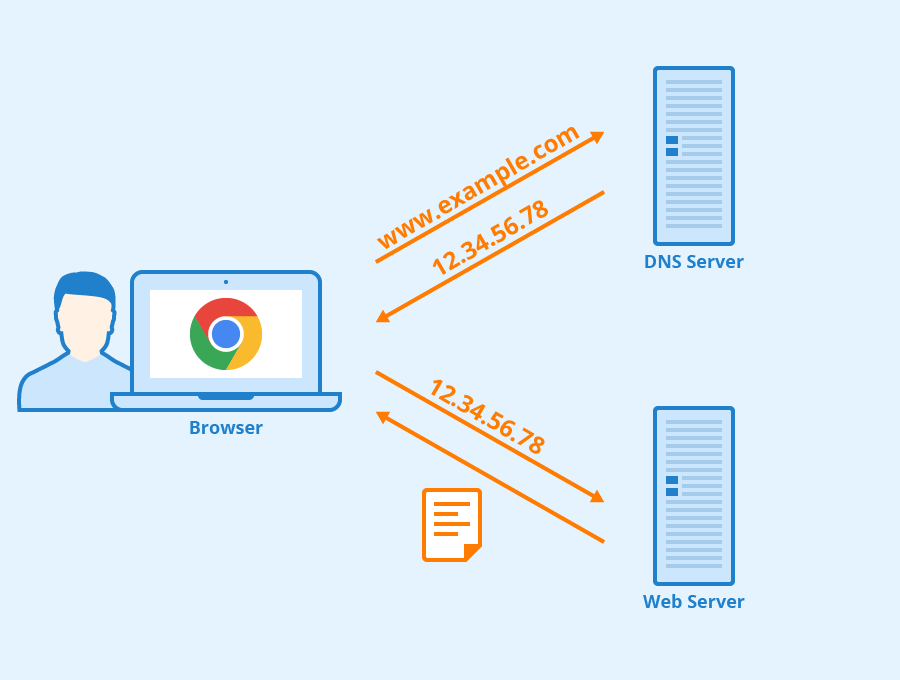
\includegraphics[width=0.5\linewidth]{State of the Art/DNS.png}
    \caption{DNS Requests and IP}
    \label{fig:enter-label}
\end{figure}
 

Originally implemented to stop email spam, Internet Protocol (IP) blocking is one of the most straightforward censorship techniques. Each device connected to the internet is assigned a unique numeric label called an IP Address, which serves as an identifier that allows data to travel across the internet to the correct destination. When a government or ISP wants to censor a specific website it can be implemented in either incoming or outgoing traffic. ISP controlled firewalls can be configured so that any outgoing or incoming requests to a selected IP address are dropped. ISPs can also adjust routing tables in their network to remove an IP address, making it unreachable for the user. 

IP blocking can either be implemented at a centralized level or at an ISP level. In Ireland, IP blocking is done at an ISP level to block certain illegal websites. The primary motivation for the Irish government in doing this is to crack down on piracy. 

DNS blocking refers to the altering of responses from the DNS to block or filter access to certain content. This is usually done by either blocking the response, replying with an error message, or responding with an incorrect address. \textit{DNS Mangling} is a network-level technique of on-path interceptioon where an incorrect IP address is returned in response to a DNS query to a censored destination. Broadly, DNS manipulation involves redirecting users by returning incorrect IP addresses. This is used to route users to controlled versions of websites or block access entirely and thus is covert in nature.

\textit{DNS Cache Poisoning} is an off-path technique in which a censor intercepts and replaces the legitimate response from an authoritative DNS name server with a spoofed IP address. Instead of allowing the real IP address of a site to reach the user, the censor replies faster than the real server, and that spoofed IP gets cached (perhaps by numerous recursive resolvers). Subsequent requests will then be redirected to an incorrect IP, normally leading to a warning page or an meaningless domain. In other cases, such as in Iran, the censor can merely block the response of the upstream resolver, so the accurate IP address is never transmitted.

\textit{DNS Lying} is the most authoritative approach, where a censor mandates that the DNS responses provided are to be different that what would actually be returned by the DNS server \cite{rfc9505}.

\subsection{Transport Layer Security (TLS) (Griff)}

Transport Layer Security (TLS) may be censored by mechanisms similar to those against plain HTTP, particularly through the Server Name Indication (SNI) field. In the case of TLS over TCP, the SNI value is seen in the non-encrypted ClientHello message so that censors can inspect the field and exclude connections to those domains they disapprove of. While QUIC encrypts ClientHello, the initial encryption keys are visible to network observers, and therefore it is possible, though more complex, to decrypt and observe the SNI. Governments in most nations use SNI-based filtering, occasionally leading to over-blocking when important domains or second-level domains are inadvertently ensnared.

Attempts to encrypt SNI have resulted in Encrypted SNI (ESNI), which embeds the SNI field in encrypted traffic but can induce blanket blocking by censors who blindly terminate all ESNI connections. Even more comprehensive security improvements, such as Encrypted Client Hello (ECH) for TLS 1.3, aim to encrypt the whole ClientHello rather than merely the SNI, though these enhancements are still under way in standardization and deployment.

Another way is to not include the SNI at all. However, non-SNI connections can be blocked as well, since censors can deploy policies that will drop any TLS traffic that does not have an SNI. This can again lead to overblocking, since clients that are able to handle older SSL-only configurations, or are deliberately configured not to have an SNI, can get blocked even when they are going to otherwise acceptable sites.

Censors also have the option to examine the server certificate field within the TLS handshake, which contains information on the requested domain. In TLS 1.3, however, certificates are encrypted by default, and thus such censorship is not possible. Certificate-inspecting censors must therefore employ more computation-intensive deep packet inspection techniques and can even be forced to track connections deeper into the handshake process, especially when SNI-based approaches fail or bypassed \cite{rfc9505}.

\subsection{MITM Attacks}
Kampourakis, Kambourakis, Chatzoglou, and Zaroliagis wrote an academic paper in 2022 arguing the effectiveness of MITM attacks against HTTPS in certain circumstance. They describe a MITM attack as follows. 
"A man-in-the-middle (MitM) attack enables threat actors to position themselves in a conversation between two parties. It can be used to eavesdrop on, or impersonate, either of the parties and may enable the perpetrator to steal personal information, including login credentials, payment card data and account details."\cite{MITMvHTTPS}

A man-in-the-middle attack involves intercepting encrypted packets (potentially at a point of control), to alter or block internet traffic. Governments have been seen to pressure VPNs into routing traffic through designated MITM servers. Inevitably this allows for selective content manipulation, deep packet inspection and surveillance. MITM attacks are particularly concerning due to their covert and intrusive nature. 

RFC 2818, released in 2000, describes "how to use TLS to secure HTTP connections over the Internet," \cite{rfc2818}known as HTTPS. This was designed to mitigate the effects of MITM attacks. Recent research suggests deployments of HTTPS in most browsers is insecure, at least in certain circumstance. Kampourakis and his colleagues went on to say "some insidious variants of MitM against HTTPS remain quite realistic across all popular Internet browser types irrespective of the underlying platform." \cite{MITMvHTTPS} 
They mention how "both of the attack variations were successful against all the browser types and versions..." except the latest versions of Firefox that they tested.

\section{Content Manipulation}
Beyond IP and DNS manipulation, censors can examine the contents within packets to make decisions regarding their accessibility. This refers to the concept of application layer filtering or blocking; monitoring a communication channel and detecting offensive keywords. This is seen in more cultivated censorship models. Upon detecting a sensitive keyword, the communication will be disrupted, perhaps by sending TCP reset packets to both sides.

\subsection{Keyword Filtering}
Keyword filtering involves 

\subsection{Deep Packet Inspection}

Deep packet inspection involves looking into payloads and data within packets, beyond its header. It is a sophisticated technique usually performed as part of a firewall defense and involves making real time decisions about the nature of each packet. DPI functions at the application level and can be used to identify both the sender and recipient of the packet by examining its payload. Compared to regular packet inspection which is only concerned with basic header information, it is considerably more costly. 

Deep packet inspection is used in specific cases where a higher level of audit is required. This includes packets carrying malware, content that has been blocked and intrusion efforts. DPI is usually performed by network middle boxes, devices that lie between end points. One of the these middle boxes is BlindBox, a system that accommodates DPI while preserving privacy and encryption. The creators of this system highlight the potential risks to user privacy with other black boxes. "To enable middlebox processing, some currently deployed middlebox systems support HTTPS in
an insecure way: they mount a man-in-the-middle attack on SSL and decrypt the traffic at the middlebox." \cite{sherry2015blindbox}

Though its deployment is limited, DPI represents a significant risk to user privacy. Not all middle box providers offer the protections and guarantees that BlindBox offer. Forecasts for the market show a troubling trend, with no guarantees of user privacy. "Global deep packet inspection (DPI) market size was anticipated to be worth USD 10.63 billion in 2024 and is expected to reach USD 79.26 billion by 2033 at a CAGR of 25\% during the forecast period." \cite{DPIMarketInfo}

\section{Legislative and Economic Pressure}
Governments can enforce censorship directly through ISPs, tech companies and social media platforms by creating new legislation or simply mandating content be removed. This is used to de-platform individuals and movements during periods of unrest. This is also done in app stores, shutting down entire platforms that are deemed problematic.

\subsection{Search Engine Manipulation}

Altering the ranking of websites or totally removing them from search results. This is done by companies like Google to incentivise paying for exposure, to censor content for compliance reasons, improve user experience and more. 


\section{Surveillance and Deanonymisation}

In discussing internet user rights and how censorship occurs, it is important to mention anonymity and user privacy. DRI, a non-profit that challenges the Irish government on data retention issues is an independent, non-profit organization. They state on their website, that users have "a right to digital privacy [\&] data security." \cite{digital_rights_ireland} Individuals' freedom to access information and be anonymous are inherently linked, however very separate issues. Though censors may actively engage in deanonymisation efforts, potentially using methods described below, this research is focused on internet censorship. Hence, deanonymisation and surveillance will only be touched on briefly.

Efforts to identify users based on their traffic range from trivial to extremely complex based upon the protections employed by the user. Operational security, the collection of measures taken by an individual to protect their online anonymity, is often overlooked by casual internet users. Projects like Tor, Tails OS (an amnesiac Linux distribution), and Briar (secure off-grid communication) as well as VPNs aim to protect users’ identity. However, these methods are not fool proof. 

VPN providers are subject to the scrutiny of the jurisdiction within which it operates. NordVPN, a very popular VPN provider based in Amserdam has said on record "We will comply with lawful requests as long as they are delivered according to all the laws and regulations." This reflects the reality of VPN services as provided by corporations. VPNs in this sense can be described as a double edged sword. In most cases they are very helpful in protecting user anonymity and circumventing censorship. However, if legislative pressure is applied, corporations will have no choice but to comply with the demands of the government. This may be trivial and to be expected by most consumers of VPN services, however, security issues in open source and previously trusted projects like TOR represent a more grave concern. 

\subsection{Side Channel Attacks}
Previously, it was touched on that German authorities managed to de anonymise Tor users by deploying timing attacks. This was a concerning development in 2022 as basic internet privacy was called into question. Users assume taking measures like using Tor would provide robust privacy guarantees; however, as of late this has been undermined by several tactics used by adversaries around the globe. Side-channel attacks, for example, are are used and are quite costly. One example of this is timing attacks. This involves correlating the time taken for a computer to perform a task or perhaps how much energy was used, with what that task might be. These attacks are based on physical phenomena experienced by electronic parts such as power consumption in CMOS devices. These attacks are typically used to crack keys, voiding unprotected implementations of cryptographic primitives such as DES (Data Encryption Standard).

Standaert, when discussing side channel attacks mentions two ways of looking at a cryptographic primitive. One could view it as a black box, some mathematical functions that translates inputs to outputs. However, another approach could be to consider how this black box will "have to be implemented in a program that will run on a given processor, in a given environment, and will therefore present specific characteristic." \cite{standaert2005introduction} 

